\chapter{Cinética química: leis de velocidade}\label{ch:b1:rate-laws}

O leite se conserva uma semana na geladeira e um dia sobre uma mesa de
verão. A caixa de um medicamento diz ``conservar abaixo de
\qty{25}{\celsius}'' e traz um prazo de validade de dois ou três anos à
frente, que o fabricante não teve tempo de observar diretamente. As
constantes de equilíbrio dizem onde uma reação termina; não dizem nada
sobre quanto tempo ela leva para chegar lá. Esse é o domínio da cinética
química. Este capítulo define a velocidade de uma reação, as \omterm{def:b1:rate-laws:order}{leis de
velocidade} que a expressam em função das concentrações, as formas
integradas que preveem as concentrações em qualquer instante, os
métodos experimentais que determinam uma \omterm{def:b1:rate-laws:order}{lei de velocidade} e a \omterm{thm:b1:rate-laws:arrhenius}{lei de
Arrhenius}, que descreve o efeito da temperatura --- a ferramenta com que
se prevê o prazo de validade de um medicamento em algumas semanas de
experimentos.

\begin{recall}
O Livro 1 (ano 12) apresentou a velocidade de aparecimento e de
desaparecimento de uma espécie, os fatores cinéticos (concentração,
temperatura, catalisador) e a \omterm{def:b1:rate-laws:half-life}{meia-vida} de uma reação de primeira ordem.
O avanço $\xi$ de uma reação foi definido na
\cref{def:b1:extent-q-and-k:extent}.
\end{recall}

\begin{omfigure}
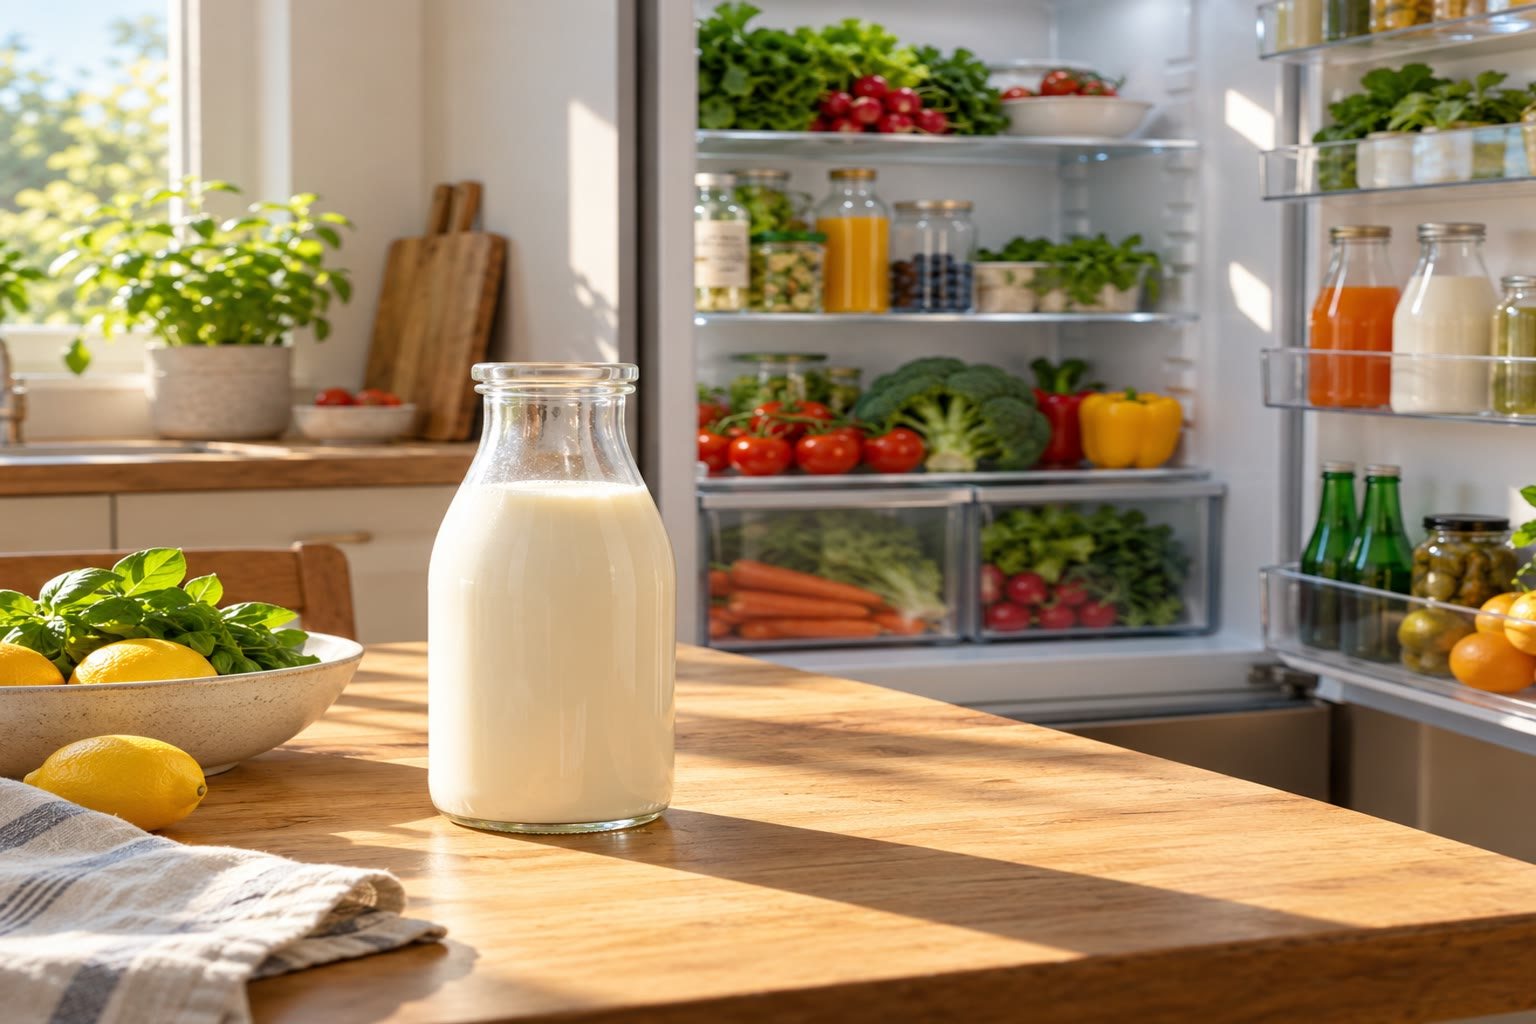
\includegraphics[width=0.55\linewidth]{images/book2/ai/b1-08-milk-kitchen.jpg}

{\small Uma garrafa de leite deixada ao sol ao lado de uma geladeira
aberta. As reações que o estragam são várias vezes mais rápidas à
temperatura do verão do que no frio.}
\end{omfigure}

\section{A velocidade de uma reação}

\begin{definition}[Velocidade de reação, velocidades de formação e de desaparecimento]\label{def:b1:rate-laws:rate}
Para uma reação $0 = \sum_i \nu_i\mathrm{A}_i$ que ocorre em um reator
fechado de volume constante $V$, a \emph{velocidade de reação}\index{velocidade de reacao@velocidade de reação}
é
\[
  v = \frac{1}{V}\frac{\dd\xi}{\dd t} = \frac{1}{\nu_i}\frac{\dd[\mathrm{A}_i]}{\dd t}
  \quad\text{(qualquer } i\text{)},
\]
em \unit{mol.L^{-1}.s^{-1}}. A \emph{velocidade de formação}\index{velocidade de formacao@velocidade de formação}
de um produto é $\dd[\mathrm{A}_i]/\dd t$; a \emph{velocidade de
desaparecimento}\index{velocidade de desaparecimento} de um reagente é
$-\dd[\mathrm{A}_i]/\dd t$.
\end{definition}

\begin{proposition}[Uma única velocidade para todas as espécies]\label{prop:b1:rate-laws:rate-relations}
A \omterm{def:b1:rate-laws:rate}{velocidade de reação} não depende da espécie escolhida para
acompanhá-la: para $a\,\mathrm{A} + b\,\mathrm{B} \longrightarrow c\,\mathrm{C} + d\,\mathrm{D}$,
\[
  v = -\frac1a\frac{\dd[\ce{A}]}{\dd t} = -\frac1b\frac{\dd[\ce{B}]}{\dd t}
  = \frac1c\frac{\dd[\ce{C}]}{\dd t} = \frac1d\frac{\dd[\ce{D}]}{\dd t} .
\]
\end{proposition}

\begin{proof}
$[\mathrm{A}_i] = (n_{i,0} + \nu_i\xi)/V$ com $V$ constante, logo
$\dd[\mathrm{A}_i]/\dd t = (\nu_i/V)\,\dd\xi/\dd t = \nu_i v$.
\end{proof}

\begin{example}[Decomposição do pentóxido de dinitrogênio]\label{ex:b1:rate-laws:n2o5}
Para \ce{2N2O5 -> 4NO2 + O2}: $v = -\frac12\frac{\dd[\ce{N2O5}]}{\dd t} =
\frac14\frac{\dd[\ce{NO2}]}{\dd t} = \frac{\dd[\ce{O2}]}{\dd t}$. O dióxido
de nitrogênio aparece quatro vezes mais depressa que o dioxigênio, e o
pentóxido de dinitrogênio desaparece duas vezes mais depressa do que o
dioxigênio aparece.
\end{example}

\section{Leis de velocidade e ordens}

\begin{definition}[Lei de velocidade, ordens, constante de velocidade]\label{def:b1:rate-laws:order}
Uma \emph{lei de velocidade}\index{lei de velocidade} exprime a velocidade
em função das concentrações. Uma reação \emph{admite uma ordem} quando
sua lei de velocidade tem a forma
\[
  v = k\,[\mathrm{A}]^{p}\,[\mathrm{B}]^{q} \cdots ;
\]
os expoentes $p$, $q$, \dots\ são as \emph{ordens parciais}\index{ordem parcial}
em relação a A, B, \dots, sua soma é a \emph{ordem
global}\index{ordem global}, e $k$ é a \emph{constante de velocidade}\index{constante de velocidade},
que só depende da temperatura. As ordens são determinadas
experimentalmente; não precisam ser iguais aos coeficientes
estequiométricos e podem ser fracionárias ou nulas.
\end{definition}

\begin{remark}[Unidades de $k$]\label{rem:b1:rate-laws:units}
Como $v$ está em \unit{mol.L^{-1}.s^{-1}}, $k$ está em
\unit{mol.L^{-1}.s^{-1}} para a ordem 0, em \unit{s^{-1}} para a ordem 1,
em \unit{L.mol^{-1}.s^{-1}} para a ordem 2 e, em geral, em
$(\unit{mol/L})^{1-n}\,\unit{s^{-1}}$ para a \omterm{def:b1:rate-laws:order}{ordem global} $n$. A unidade
de $k$ indica a \omterm{def:b1:rate-laws:order}{ordem global}.
\end{remark}

\begin{remark}[Reações sem ordem]\label{rem:b1:rate-laws:no-order}
Nem toda reação admite uma ordem. A velocidade de algumas reações é uma
fração cujo denominador contém concentrações, ou depende da concentração
de um produto. Essas \omterm{def:b1:rate-laws:order}{leis de velocidade} são explicadas pelo mecanismo da
reação (\cref{ch:b1:elementary-steps}). Uma reação também pode admitir
uma ordem apenas no início: a lei de \omterm{def:b1:rate-laws:initial-rate}{velocidade inicial}.
\end{remark}

\section{Leis de velocidade integradas e meias-vidas}

\begin{definition}[Meia-vida]\label{def:b1:rate-laws:half-life}
A \emph{meia-vida}\index{meia-vida} $t_{1/2}$ de um reagente é o tempo
ao fim do qual metade de sua quantidade inicial foi consumida.
\end{definition}

\begin{theorem}[Leis de velocidade integradas]\label{thm:b1:rate-laws:integrated}
Para uma reação $a\mathrm{A} \rightarrow \text{produtos}$ de velocidade $v = -\frac1a\frac{\dd[\ce{A}]}
{\dd t} = k[\ce{A}]^n$, com $[\ce{A}](0) = a_0$:
\begin{center}
\begin{tabular}{llll}
\hline
ordem & lei integrada & gráfico linear & \omterm{def:b1:rate-laws:half-life}{meia-vida} \\
\hline
0 & $[\ce{A}] = a_0 - akt$ & $[\ce{A}]$ em função de $t$ & $a_0/(2ak)$ \\
1 & $[\ce{A}] = a_0\,\eu^{-akt}$ & $\ln[\ce{A}]$ em função de $t$ & $\ln2/(ak)$ \\
2 & $\dfrac{1}{[\ce{A}]} = \dfrac{1}{a_0} + akt$ & $1/[\ce{A}]$ em função de $t$ & $1/(ak\,a_0)$ \\
\hline
\end{tabular}
\end{center}
\end{theorem}

\begin{proof}
Escreva $c = [\ce{A}]$, de modo que $\dd c/\dd t = -akc^n$.
\emph{Ordem 0}: $\dd c/\dd t = -ak$, logo $c = a_0 - akt$ (válida até
$c = 0$). \emph{Ordem 1}: $\dd c/\dd t = -akc$ é uma equação diferencial
linear de primeira ordem cuja solução é $c = a_0\eu^{-akt}$.
\emph{Ordem 2}: $\dd c/c^2 = -ak\,\dd t$; integrando de 0 a $t$,
$-1/c + 1/a_0 = -akt$, logo $1/c = 1/a_0 + akt$. Meias-vidas: faça $c =
a_0/2$ em cada lei e resolva em $t$.
\end{proof}

\begin{proposition}[O teste da meia-vida]\label{prop:b1:rate-laws:half-life-test}
A \omterm{def:b1:rate-laws:half-life}{meia-vida} é independente da concentração inicial se e somente se a
reação for de ordem 1. Ela é proporcional a $a_0$ para a ordem 0 e a
$1/a_0$ para a ordem 2. Uma reação de primeira ordem perde a metade do
que resta a cada \omterm{def:b1:rate-laws:half-life}{meia-vida} sucessiva: depois de $m$ meias-vidas, resta
uma fração $2^{-m}$.
\end{proposition}

\begin{proof}
Para a ordem $n \ne 1$, a separação de variáveis dá $t_{1/2} = \dfrac{2^{n-1} -
1}{(n-1)\,ak\,a_0^{n-1}}$, que depende de $a_0$, a menos que $n = 1$; para
$n = 1$, $t_{1/2} = \ln2/(ak)$. Para a ordem 1, $c(t + t_{1/2}) = c(t)/2$
em todo $t$, pois $\eu^{-ak(t + t_{1/2})} = \eu^{-akt}/2$.
\end{proof}

\begin{omfigure}
\begin{tikzpicture}
\begin{axis}[name=p0,
  width=0.36\linewidth, height=4.6cm,
  xmin=0, xmax=60, ymin=0, ymax=1.05,
  axis x line=bottom, axis y line=left,
  xlabel={$t$ (min)}, title={ordem 0: $[\ce{A}]$},
  title style={font=\small}, xtick={0,20,40,60},
  tick label style={font=\scriptsize}, label style={font=\small}]
\addplot[omDef, thick] table[x=t, y=A0] {figdata/out/bachelor-1-integrated-rate-laws.dat};
\end{axis}
\begin{axis}[at={(p0.east)}, anchor=west, xshift=0.9cm, name=p1,
  width=0.36\linewidth, height=4.6cm,
  xmin=0, xmax=60, ymin=-3.2, ymax=0.2,
  axis x line=bottom, axis y line=left,
  xlabel={$t$ (min)}, title={ordem 1: $\ln[\ce{A}]$},
  title style={font=\small}, xtick={0,20,40,60},
  tick label style={font=\scriptsize}, label style={font=\small}]
\addplot[omProp, thick] table[x=t, y=lnA1] {figdata/out/bachelor-1-integrated-rate-laws.dat};
\end{axis}
\begin{axis}[at={(p1.east)}, anchor=west, xshift=0.9cm,
  width=0.36\linewidth, height=4.6cm,
  xmin=0, xmax=60, ymin=0, ymax=4.2,
  axis x line=bottom, axis y line=left,
  xlabel={$t$ (min)}, title={ordem 2: $1/[\ce{A}]$},
  title style={font=\small}, xtick={0,20,40,60},
  tick label style={font=\scriptsize}, label style={font=\small}]
\addplot[omThm, thick] table[x=t, y=invA2] {figdata/out/bachelor-1-integrated-rate-laws.dat};
\end{axis}
\end{tikzpicture}

\begin{tikzpicture}
\begin{axis}[
  width=0.62\linewidth, height=5.0cm,
  xmin=0, xmax=60, ymin=0, ymax=1.05,
  axis x line=bottom, axis y line=left,
  xlabel={$t$ (min)}, ylabel={$[\ce{A}]$ (mol/L)}, xtick={0,10,20,30,40,50,60},
  tick label style={font=\small}, label style={font=\small},
  legend style={font=\small, draw=none, at={(0.98,0.98)}, anchor=north east}]
\addplot[omDef, thick] table[x=t, y=A0] {figdata/out/bachelor-1-integrated-rate-laws.dat};
\addplot[omProp, thick] table[x=t, y=A1] {figdata/out/bachelor-1-integrated-rate-laws.dat};
\addplot[omThm, thick] table[x=t, y=A2] {figdata/out/bachelor-1-integrated-rate-laws.dat};
\legend{ordem 0, ordem 1, ordem 2}
\draw[dotted] (axis cs:0,0.5) -- (axis cs:20,0.5);
\end{axis}
\end{tikzpicture}

{\small Três reações com a mesma concentração inicial
(\qty{1.00}{mol/L}) e a mesma \omterm{def:b1:rate-laws:initial-rate}{velocidade inicial}
(\qty{0.050}{mol.L^{-1}.min^{-1}}). Em cima: cada lei integrada vira uma
reta em suas próprias coordenadas. Embaixo: as concentrações; as
meias-vidas são de 10, 13.9 e 20 minutos.}
\end{omfigure}

\section{Determinar uma lei de velocidade}

\begin{method}[O método integral]\label{met:b1:rate-laws:integral}
Para testar uma ordem com medidas de $[\ce{A}](t)$: trace $[\ce{A}]$,
$\ln[\ce{A}]$ e $1/[\ce{A}]$ em função de $t$; o gráfico que for uma reta
dá a ordem, e sua inclinação dá $k$ (inclinação $-ak$, $-ak$ ou $+ak$,
respectivamente).
\end{method}

\begin{method}[O método da meia-vida]\label{met:b1:rate-laws:half-life}
Meça a \omterm{def:b1:rate-laws:half-life}{meia-vida} para várias concentrações iniciais: constante, ordem 1;
proporcional a $a_0$, ordem 0; proporcional a $1/a_0$, ordem 2. Em um
único experimento, compare os tempos para ir de $a_0$ a $a_0/2$ e de
$a_0/2$ a $a_0/4$: tempos iguais indicam ordem 1.
\end{method}

\begin{definition}[Velocidade inicial]\label{def:b1:rate-laws:initial-rate}
A \emph{velocidade inicial}\index{velocidade inicial} $v_0$ é a velocidade
em $t = 0$, lida como a inclinação da tangente na origem à curva
$[\ce{A}](t)$, dividida pelo coeficiente estequiométrico. Nesse instante,
as concentrações são as iniciais, conhecidas, e nenhum produto interfere.
\end{definition}

\begin{method}[O método das velocidades iniciais]\label{met:b1:rate-laws:initial-rates}
Para $v_0 = k[\ce{A}]_0^p[\ce{B}]_0^q$: faça experimentos variando apenas
$[\ce{A}]_0$; então $\ln v_0 = \ln(k[\ce{B}]_0^q) + p\ln[\ce{A}]_0$, e a
inclinação de $\ln v_0$ em função de $\ln[\ce{A}]_0$ é $p$. Na prática,
dobrar $[\ce{A}]_0$ multiplica $v_0$ por $2^p$. Faça o mesmo para B.
\end{method}

\begin{definition}[Método do isolamento, ordem aparente]\label{def:b1:rate-laws:apparent-order}
No \emph{método do isolamento}\index{metodo do isolamento@método do isolamento}, todos os reagentes,
exceto um, são colocados em grande excesso (dez vezes ou mais). Suas
concentrações ficam praticamente constantes, e $v = k[\ce{A}]^p[\ce{B}]^q \approx k'[\ce{A}]^p$
com $k' = k[\ce{B}]_0^q$: a reação se comporta como se fosse de
\emph{ordem aparente}\index{ordem aparente} $p$, com a \omterm{def:b1:rate-laws:order}{constante de
velocidade} aparente $k'$. Fala-se também em degenerescência da ordem.
\end{definition}

\begin{omfigure}
\begin{tikzpicture}
\begin{axis}[
  width=0.55\linewidth, height=4.8cm,
  xmin=0, xmax=40, ymin=0, ymax=1.05,
  axis x line=bottom, axis y line=left,
  xlabel={$t$ (min)}, ylabel={$[\ce{A}]$ (mol/L)},
  xtick={0,10,20,30,40},
  tick label style={font=\small}, label style={font=\small}, clip mode=individual]
\addplot[omProp, thick] table[x=t, y=A1] {figdata/out/bachelor-1-integrated-rate-laws.dat};
\draw[omThm, thick] (axis cs:0,1) -- (axis cs:20,0);
\node[omThm, anchor=west, font=\small] at (axis cs:2,0.12) {\shortstack[r]{tangente\\em $t = 0$}};
\end{axis}
\end{tikzpicture}

{\small Leitura de uma \omterm{def:b1:rate-laws:initial-rate}{velocidade inicial}: a tangente na origem (em
vermelho) a uma curva de primeira ordem corta o eixo dos tempos em
$t_0 = \qty{20}{min}$, logo $v_0 =
\qty{1.00}{mol/L}/\qty{20}{min} = \qty{0.050}{mol.L^{-1}.min^{-1}}$.}
\end{omfigure}

\begin{inthelab}[Acompanhar uma reação no tempo]
Uma \omterm{def:b1:rate-laws:order}{lei de velocidade} é construída a partir de concentrações medidas
enquanto a reação ocorre. Quando um reagente ou um produto é colorido, um
espectrofotômetro registra a absorbância, proporcional à sua
concentração (Beer--Lambert, \cref{ch:b1:structure-spectroscopy});
quando íons aparecem ou desaparecem, um condutivímetro acompanha a
condutividade; quando se forma um gás em um recipiente fechado, um
manômetro acompanha a pressão. Caso contrário, retiram-se amostras em
instantes conhecidos, a reação é bloqueada por resfriamento ou diluição,
e cada amostra é titulada. A temperatura do recipiente é mantida
constante por um banho termostatizado, porque $k$ depende fortemente
dela.
\end{inthelab}

\section{A temperatura: a lei de Arrhenius}

\begin{definition}[Energia de ativação]\label{def:b1:rate-laws:activation-energy}
A \emph{energia de ativação}\index{energia de ativacao@energia de ativação} $E_a$ de uma reação
de \omterm{def:b1:rate-laws:order}{constante de velocidade} $k(T)$ é definida por
\[
  \frac{\dd \ln k}{\dd T} = \frac{E_a}{RT^2} ,
\]
em \unit{J/mol}. Quando $E_a$ é independente de $T$, a integração dá
$k = A\,\eu^{-E_a/RT}$, em que a constante $A$, com a unidade de $k$, é
o \emph{fator pré-exponencial}\index{fator pre-exponencial@fator pré-exponencial}.
\end{definition}

\begin{theorem}[Lei de Arrhenius]\label{thm:b1:rate-laws:arrhenius}
Para a maioria das reações, em um intervalo moderado de temperatura, a
\omterm{def:b1:rate-laws:order}{constante de velocidade} segue a \emph{lei de Arrhenius}\index{lei de Arrhenius}
\[
  k(T) = A\,\eu^{-E_a/RT} ,
\]
com $A$ e $E_a > 0$ independentes de $T$: $\ln k$ é uma função afim de
$1/T$, de inclinação $-E_a/R$.
\end{theorem}
\admitted

\begin{remark}[O significado de $E_a$]\label{rem:b1:rate-laws:meaning}
A lei é empírica. Sua interpretação --- só as colisões moleculares que
trazem pelo menos uma energia da ordem de $E_a$ levam à reação, e a
fração dessas colisões varia como $\eu^{-E_a/RT}$ --- é esboçada com os
perfis de energia do próximo capítulo e tornada quantitativa pelas
teorias das \omterm{def:b1:rate-laws:rate}{velocidades de reação} no volume do 3.º ano.
\end{remark}

\begin{method}[Determinar $E_a$]\label{met:b1:rate-laws:arrhenius-plot}
A partir de \omterm{def:b1:rate-laws:order}{constantes de velocidade} a várias temperaturas, trace $\ln k$
em função de $1/T$ (em kelvin): a inclinação é $-E_a/R$, o coeficiente
linear é $\ln A$. Com apenas duas temperaturas,
\[
  E_a = \frac{R\,\ln(k_2/k_1)}{1/T_1 - 1/T_2} .
\]
\end{method}

\begin{example}[Uma regra prática]\label{ex:b1:rate-laws:doubling}
Para $E_a = \qty{53}{kJ/mol}$, passar de 25 a \qty{35}{\celsius}
multiplica $k$ por $\exp\!\big(\frac{53000}{8.314}(\frac{1}{298.15} -
\frac{1}{308.15})\big) = 2.0$. A regra conhecida ``dez graus a mais, duas
vezes mais rápido'' vale perto da temperatura ambiente para reações de
\omterm{def:b1:rate-laws:activation-energy}{energia de ativação} em torno de \qty{50}{kJ/mol}; para $E_a$ maiores, o
fator é maior.
\end{example}

\begin{omfigure}
\begin{tikzpicture}
\begin{axis}[
  width=0.6\linewidth, height=5.4cm,
  xmin=2.95, xmax=3.45, ymin=-9.0, ymax=-4.2, clip mode=individual,
  axis x line=bottom, axis y line=left,
  xlabel={$1000/T$ (\unit{K^{-1}})}, ylabel={$\ln k$ ($k$ em \unit{d^{-1}})},
  xtick={3.0,3.1,3.2,3.3,3.4}, ytick={-9,-8,-7,-6,-5},
  tick label style={font=\small}, label style={font=\small}]
\addplot[omDef, thick] table[x=invT_1e3, y=lnk] {figdata/out/bachelor-1-arrhenius-line.dat};
\addplot[only marks, mark=*, mark size=2.2pt, omThm] table[x=invT_1e3, y=lnk] {figdata/out/bachelor-1-arrhenius-points.dat};
\node[font=\small, anchor=south west] at (axis cs:3.002,-4.71) {\qty{60}{\celsius}};
\node[font=\small, anchor=south west] at (axis cs:3.095,-5.66) {\qty{50}{\celsius}};
\node[font=\small, anchor=south west] at (axis cs:3.193,-6.67) {\qty{40}{\celsius}};
\draw[dashed, black!50] (axis cs:3.354,-9.0) -- (axis cs:3.354,-8.31);
\addplot[only marks, mark=o, mark size=2.4pt, omDef] coordinates {(3.354,-8.310)};
\node[font=\small, anchor=east] at (axis cs:3.33,-8.40) {\qty{25}{\celsius}, extrapolado};
\end{axis}
\end{tikzpicture}

{\small Gráfico de Arrhenius da degradação de um medicamento (problema de
fim de semana): três \omterm{def:b1:rate-laws:order}{constantes de velocidade} medidas (em vermelho)
ficam sobre uma reta de inclinação $-E_a/R$; extrapolada para
\qty{25}{\celsius}, ela dá o prazo de validade à temperatura ambiente.}
\end{omfigure}

\begin{history}[Arrhenius, 1889]
O químico sueco Svante Arrhenius, estudando a inversão da sacarose pelos
ácidos em 1889, propôs que só uma pequena fração das moléculas, as que
estão em um estado ``ativado'', reage, e que essa fração cresce com a
temperatura como $\eu^{-E/RT}$. A ideia, controversa no início, tornou-se
o fundamento da cinética química. Arrhenius recebeu o Prêmio Nobel de
Química em 1903, por sua teoria da dissociação eletrolítica.
\end{history}

\begin{omfigure}
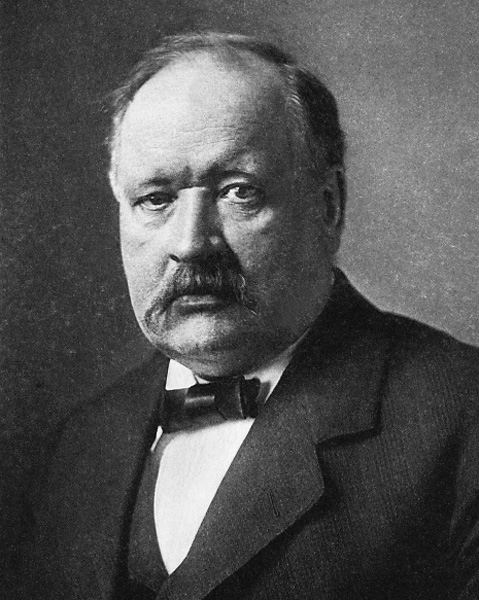
\includegraphics[width=0.22\linewidth]{images/book2/arrhenius.jpg}

{\small Svante Arrhenius (1859--1927), em 1909.}
\end{omfigure}

\section{Exercícios}

\begin{exercise}[$\star$]\label{exo:b1:rate-laws:1}
Para \ce{2N2O5 -> 4NO2 + O2} a volume constante, o dióxido de nitrogênio
aparece a $\qty{2.0e-4}{mol.L^{-1}.s^{-1}}$. Dê a \omterm{def:b1:rate-laws:rate}{velocidade de reação},
a \omterm{def:b1:rate-laws:rate}{velocidade de formação} do dioxigênio e a \omterm{def:b1:rate-laws:rate}{velocidade de desaparecimento}
de \ce{N2O5}.
\end{exercise}

\begin{exercise}[$\star$]\label{exo:b1:rate-laws:2}
Dê a unidade da \omterm{def:b1:rate-laws:order}{constante de velocidade} para as \omterm{def:b1:rate-laws:order}{ordens globais} 0, 1, 2 e
3, com as concentrações em \unit{mol/L} e os tempos em segundos.
\end{exercise}

\begin{exercise}[$\star$]\label{exo:b1:rate-laws:3}
Uma reação de primeira ordem $\mathrm{A} \longrightarrow \mathrm{B}$ tem $k = \qty{3.0e-3}{s^{-1}}$.
Calcule sua \omterm{def:b1:rate-laws:half-life}{meia-vida} e a fração de \ce{A} restante após \qty{10}{min}.
\end{exercise}

\begin{exercise}[$\star$]\label{exo:b1:rate-laws:4}
Quando a concentração inicial de um reagente é reduzida à metade, sua
\omterm{def:b1:rate-laws:half-life}{meia-vida} dobra. Qual é a ordem? E se a \omterm{def:b1:rate-laws:half-life}{meia-vida} se reduzir à metade?
\end{exercise}

\begin{exercise}[$\star\star$]\label{exo:b1:rate-laws:5}
Mede-se a concentração de um reagente \ce{A} ($\mathrm{A} \longrightarrow \mathrm{P}$): em $t
= 0$, 10, 20, 30 e \qty{40}{min}, $[\ce{A}] = 0.100$, 0.0741, 0.0549,
0.0407 e \qty{0.0301}{mol/L}. Determine a ordem e a \omterm{def:b1:rate-laws:order}{constante de
velocidade}.
\end{exercise}

\begin{exercise}[$\star\star$]\label{exo:b1:rate-laws:6}
Para $\mathrm{A} + \mathrm{B} \longrightarrow \mathrm{P}$, $v_0 = \qty{2.0e-6}{mol.L^{-1}.s^{-1}}$ para $[\ce{A}]_0
= [\ce{B}]_0 = \qty{0.010}{mol/L}$; \qty{8.0e-6}{} quando $[\ce{A}]_0$ é
dobrada; \qty{4.0e-6}{} quando $[\ce{B}]_0$ é dobrada. Encontre as \omterm{def:b1:rate-laws:order}{ordens
parciais}, a \omterm{def:b1:rate-laws:order}{lei de velocidade} e a \omterm{def:b1:rate-laws:order}{constante de velocidade}.
\end{exercise}

\begin{exercise}[$\star\star$]\label{exo:b1:rate-laws:7}
A \omterm{def:b1:rate-laws:order}{lei de velocidade} de $\mathrm{A} + \mathrm{B} \longrightarrow \mathrm{P}$ é $v = k[\ce{A}][\ce{B}]$. Com
$[\ce{B}]_0 = \qty{0.50}{mol/L}$ e $[\ce{A}]_0 = \qty{5.0e-3}{mol/L}$,
\ce{A} desaparece segundo uma cinética de primeira ordem, com constante
aparente de \qty{0.012}{s^{-1}}. Explique e calcule $k$.
\end{exercise}

\begin{exercise}[$\star\star$]\label{exo:b1:rate-laws:8}
Uma \omterm{def:b1:rate-laws:order}{constante de velocidade} vale \qty{1.0e-3}{s^{-1}} a \qty{300}{K} e
\qty{5.0e-3}{s^{-1}} a \qty{320}{K}. Calcule a \omterm{def:b1:rate-laws:activation-energy}{energia de ativação} e a
\omterm{def:b1:rate-laws:order}{constante de velocidade} a \qty{310}{K}.
\end{exercise}

\begin{exercise}[$\star\star$]\label{exo:b1:rate-laws:9}
A reação $2\,\mathrm{A} \longrightarrow \mathrm{P}$ tem a \omterm{def:b1:rate-laws:order}{lei de velocidade} $v = -\frac12\frac{\dd[\ce{A}]}
{\dd t} = k[\ce{A}]^2$ com $k = \qty{0.50}{L.mol^{-1}.s^{-1}}$. Partindo
de $[\ce{A}]_0 = \qty{0.020}{mol/L}$, calcule a \omterm{def:b1:rate-laws:half-life}{meia-vida} e a
concentração após \qty{100}{s}.
\end{exercise}

\begin{exercise}[$\star\star\star$]\label{exo:b1:rate-laws:10}
Para uma reação de primeira ordem, mostre que o tempo necessário para
consumir uma fração $f$ do reagente é $t_f = -\ln(1 - f)/(ak)$. Compare
os tempos para 50\,\%, 75\,\%, 90\,\% e 99.9\,\%, em meias-vidas.
\end{exercise}

\begin{exercise}[$\star\star\star$]\label{exo:b1:rate-laws:11}
Um adesivo transdérmico libera um fármaco a uma velocidade constante de
\qty{0.40}{mg/h} enquanto seu reservatório, inicialmente com
\qty{10}{mg}, não estiver vazio. Escreva a lei da quantidade restante,
dê sua ordem, sua \omterm{def:b1:rate-laws:half-life}{meia-vida} e o tempo ao fim do qual o adesivo se
esgota. Por que uma cinética de ordem zero convém a um adesivo
medicamentoso?
\end{exercise}

\begin{exercise}[$\star\star\star$]\label{exo:b1:rate-laws:12}
Mostre que a regra ``dez graus a mais, duas vezes mais rápido'' entre
\qty{298.15}{K} e \qty{308.15}{K} corresponde a $E_a \approx
\qty{53}{kJ/mol}$. Que fator a mesma \omterm{def:b1:rate-laws:activation-energy}{energia de ativação} dá entre
\qty{0}{\celsius} e \qty{10}{\celsius}?
\end{exercise}

\section{Problema: O prazo de validade de um medicamento}

\begin{problem}[{Problema de fim de semana --- um teste de estabilidade
acelerado: degradação de primeira ordem a 60\,\textdegree C, três
temperaturas, o gráfico de Arrhenius e o prazo de validade à temperatura
ambiente}]
\label{pb:b1:rate-laws:1}
Para prever o prazo de validade $t_{90}$ de um comprimido (o tempo ao
fim do qual 10\,\% do princípio ativo se degradou), um laboratório
guarda amostras a alta temperatura e mede a porcentagem de princípio
ativo restante. A
\qty{60}{\celsius}:
\begin{center}
\begin{tabular}{lccccc}
\hline
tempo (dias) & 0 & 10 & 20 & 30 & 40 \\
princípio ativo restante (\%) & 100.0 & 91.4 & 83.5 & 76.3 & 69.8 \\
\hline
\end{tabular}
\end{center}
A 40 e a \qty{50}{\celsius}, as \omterm{def:b1:rate-laws:order}{constantes de velocidade} encontradas são
\qty{1.27e-3}{d^{-1}} e \qty{3.48e-3}{d^{-1}}. Considere $R =
\qty{8.314}{J/(mol.K)}$ e um mês $= \qty{30.4}{d}$.

\medskip
\noindent\textbf{Parte I --- A ordem a 60\,\textdegree C.}
\begin{enumerate}
  \item Calcule as perdas em cada intervalo de 10 dias. A reação é de
        ordem 0?
  \item Calcule $\ln(\%\text{ restante})$ em cada instante. O que você conclui?
  \item Deduza a \omterm{def:b1:rate-laws:order}{constante de velocidade} $k_{60}$.
  \item Calcule a \omterm{def:b1:rate-laws:half-life}{meia-vida} a \qty{60}{\celsius}.
  \item Que porcentagem resta depois de 60 dias a \qty{60}{\celsius}?
  \item Calcule $t_{90}$ a \qty{60}{\celsius}.
\end{enumerate}

\medskip
\noindent\textbf{Parte II --- Prazo de validade e ordem.}
\begin{enumerate}[resume]
  \item Mostre que, para uma degradação de primeira ordem, $t_{90} = \ln(10/9)/k$.
  \item Expresse $t_{90}$ como uma fração da \omterm{def:b1:rate-laws:half-life}{meia-vida}.
  \item Por que $t_{90}$ não depende da dosagem do comprimido?
  \item Por que os laboratórios medem a degradação a alta temperatura,
        e não a \qty{25}{\celsius}?
  \item Se a degradação fosse de ordem 2 no princípio ativo, um
        comprimido duas vezes mais forte duraria mais ou menos? Explique.
\end{enumerate}

\medskip
\noindent\textbf{Parte III --- O gráfico de Arrhenius.}
\begin{enumerate}[resume]
  \item Monte uma tabela de $1/T$ e $\ln k$ para as três temperaturas.
  \item Calcule a inclinação da reta que passa pelos pontos de 40 e
        \qty{60}{\celsius}.
  \item Deduza a \omterm{def:b1:rate-laws:activation-energy}{energia de ativação}.
  \item Verifique que o ponto de \qty{50}{\celsius} está sobre a reta.
  \item Calcule o \omterm{def:b1:rate-laws:activation-energy}{fator pré-exponencial} $A$.
  \item Por qual fator a velocidade aumenta entre 25 e
        \qty{35}{\celsius}? Compare com a regra prática.
\end{enumerate}

\medskip
\noindent\textbf{Parte IV --- A temperatura ambiente.}
\begin{enumerate}[resume]
  \item Extrapole a \omterm{def:b1:rate-laws:order}{constante de velocidade} para \qty{30}{\celsius}.
  \item Calcule $t_{90}$ a \qty{30}{\celsius}, em meses.
  \item Uma caixa é esquecida três dias em um carro a \qty{60}{\celsius}.
        Que fração do princípio ativo se perde?
  \item Explique a instrução ``conservar abaixo de \qty{25}{\celsius}''.
  \item Extrapole a \omterm{def:b1:rate-laws:order}{constante de velocidade} para \qty{25}{\celsius}.
  \item Calcule o prazo de validade $t_{90}$ a \qty{25}{\celsius}, em dias
        e em meses.
\end{enumerate}
\end{problem}
